\documentclass[a4paper,12pt,french]{article}

\usepackage[cours]{../../../Style}

\begin{document}

\titre{Nombres réels}

\section{Les ensembles de nombres}

\subsection{Les entiers}

\begin{defin}
$\N$ désigne l'ensemble des entiers positifs ou nuls, appelés entiers naturels. $0$ est un entier naturel, on note $0 \in \N$. Par contre, $-3$ n'en est pas un, on note $-3 \not\in \N$.
$$ \N = \left\{ 0;1;2; \ldots \right\}$$
\end{defin}

\begin{defin}
$\Z$ désigne l'ensemble des entiers négatifs, positifs ou nuls, appelés entiers relatifs: $1 \in \Z, -2 \in \Z$ mais $0.5 \not\in \Z$.
$$ \Z = \left\{ \ldots ; -2 ; -1 ; 0 ; 1 ; 2 ; \ldots \right\}$$
\end{defin}

\begin{rmq}
Tout entier naturel est aussi un entier relatif. L'ensemble $\N$ est donc inclus dans l'ensemble $\Z$. On note $\N \subset \Z$.
\end{rmq}

\subsection{Les nombres décimaux}

\begin{defin}
Un nombre décimal est un nombre qui peut s'écrire avec un nombre fini de chiffres après la virgule. Autrement dit, un nombre décimal peut s'écrire sous la forme $\frac a {10^n}$, où $a \in \Z$ et $n \in \N$. On note $\D$ l'ensemble des nombres décimaux.
$$0.5=\frac 5 {10} \in \D,\ 1/4=0.25 \in \D,\ \frac 1 3=0.333 \ldots \not\in \D$$
\end{defin}

\rem{ Démo en annexe }

\begin{rmq}
Tout entier relatif est aussi un entier décimal: $\Z \subset \D$: Par exemple, $-1 = \frac {-1} 1 = \frac {-1} {10^0}$.
\end{rmq}

\subsection{Les nombres rationnels}

\begin{defin}
Un nombre rationnel est un nombre qui peut s'écrire sous la forme $\frac p q$, où $p$ et $q$ sont des entiers relatifs et $q$ est non nul. On note $\Q$ l'ensemble des nombres rationnels.
$$-2 = \frac {-2} 1 \in \Q,\ \frac 1 3 \in \Q,\ \frac 3 7 \in \Q,\ \sqrt 2 \not\in \Q$$
\end{defin}

\begin{prop} \saut
\begin{itemize}
\item Tout nombre rationnel non nul admet une seule écriture fractionnaire irréductible
\item Si un nombre est rationnel, alors son développement décimal est périodique à partir d'un certain rang. La réciproque est aussi vraie.
\end{itemize}
\end{prop}

\begin{ex}
$x=0.0909 \ldots$ est rationnel: $100x=9.0909 \ldots$ donc $100x - x = 9$ d'où $99x=9$ puis $x= \frac 9 {99} = \frac 1 {11}$.
\end{ex}

\begin{exercice}
Faire de même avec $x=0.1666 \ldots$: $10x=1.666 \ldots$ donc $10x-x=1.5$ et alors $9x= \frac 3 2$ puis $x= \frac 3 {18} = \frac 1 6$.
\end{exercice}

\begin{rmq}
Tout nombre décimal est aussi un nombre rationnel: $\D \subset \Q$.
\end{rmq}

\subsection{Les nombres réels}

\begin{defin}
$\R$ désigne l'ensemble des nombres connus en classe de seconde, qu'on appelle nombres réels. De plus, un nombre réel qui n'est pas rationnel est dit irrationnel.
$$ \sqrt 2, \pi, \sqrt { \sqrt { \pi } } \text{ sont irrationnels}$$
\end{defin}

\rem{Crise des irrationnels: 6ème siècle avant J.C. Leur découverte fait du bruit dans la communauté mathématiques de l'époque car les maths étaient alors considérées comme belles, parfaites}

\begin{propr}
On représente l'ensemble des nombres réels sur une droite graduée:

\begin{center}
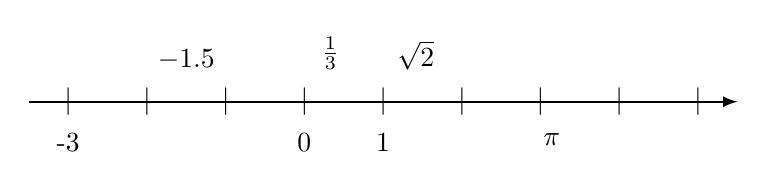
\begin{tikzpicture}[>=latex]
    \draw[thick,->] (-3.5,0) --(5.5,0);
    \node[below=8pt] at (0,0) {0};
    \node[below=8pt] at (1,0) {1};
    \node[below=8pt] at (-3,0) {-3};
    \node[above=8pt] at (1.414,0) {$\sqrt 2$};
    \node[] at (1.414,0) {$\shortmid$};
    \node[below=8pt] at (3.142,0) {$\pi$};
    \node[] at (3.142,0) {$\shortmid$};
    \node[above=8pt] at (0.33,0) {$\frac 1 3$};
    \node[] at (0.33,0) {$\shortmid$};
    \node[above=8pt] at (-1.5,0) {$-1.5$};
    \node[] at (-1.5,0) {$\shortmid$};
    \foreach \xp in {-3,-2,...,5}{\node[] at (\xp,0) {$\mid$};}
   
\end{tikzpicture}
\end{center}
\end{propr}

\begin{prop}
Tous ces ensembles sont inclus les uns dans les autres: $\N \subset \Z \subset \D \subset \Q \subset \R$.
\begin{center}
\definecolor{fond}{Hsb}{25,1,1}
\begin{tikzpicture}[xscale=1.2]
\draw[fill=fond!10!bg] (3.2,0) circle [x radius=60mm,y radius=28mm];
\draw[fill=fond!15!bg] (2.4,0) circle [x radius=50mm,y radius=25mm];
\draw[fill=fond!20!bg] (1.6,0) circle [x radius=40mm,y radius=22mm];
\draw[fill=fond!25!bg] (0.8,0) circle [x radius=30mm,y radius=19mm];
\draw[fill=fond!30!bg] (0,0) circle [x radius=20mm,y radius=16mm];

\node[font=\LARGE] at (0,0) {$\N$};
\node[] at (-1,0.5) {$0$};
\node[] at (1,0.3) {$1$};
\node[] at (-0.4,-0.9) {$3$};

\node[font=\LARGE] at (2.8,0) {$\Z$};
\node[] at (2.5,0.8) {$-2$};
\node[] at (2.6,-0.8) {$-12$};

\node[font=\LARGE] at (4.6,0) {$\D$};
\node[] at (3.8,1.4) {$0.5$};
\node[] at (4,-1) {$\dfrac 1 {10}$};

\node[font=\LARGE] at (6.4,0) {$\Q$};
\node[] at (5.9,1) {$\dfrac 1 3$};
\node[] at (5.8,-1.2) {$\dfrac {22} 7$};

\node[font=\LARGE] at (8.3,0) {$\R$};
\node[] at (7.1,-1.6) {$\pi$};
\node[] at (7.8,-1.1) {$\sqrt 2$};
\node[] at (7.6,1.2) {$\dfrac{\pi^2}6$};
\end{tikzpicture}
\end{center}
\end{prop}
\subsubsection*{Encadrement décimal des réels}

\begin{defin}
Un encadrement décimal d'un nombre réel $x$ est une écriture $d_{1}\leq x \leq d_{2}$  avec $d_{1},d_{2}$ des nombres décimaux. La différence $d_{2}-d_{1}$ est l'amplitude de l'encadrement.
\end{defin}

\begin{ex}
Par exemple, $1,4<\sqrt{2}<1,5$ est un encadrement décimal de $\sqrt{2}$ d'amplitude $10^{-1}=0.1$.
\end{ex}

\begin{defin}
Soit $x\in \R$ tel que $d_{1}\leq x\leq d_{2}$ avec $d_{2}-d_{1}=10^{-n}$ où $n\in \N$.\\L'arrondi à $10^{-n}$ de x est celui de $d_{1}$ ou $d_{2}$ le plus proche de $x$.\\Dans le cas où $d_{1}$ et $d_{2}$ sont à égale distance de $x$, l'arrondi à $10^{-n}$ de $x$ est $d_{2}$.
\end{defin}

\begin{ex}
\begin{itemize}
    \item $3,14$ est l'arrondi à $10^{-2}$ de $\pi$.
    \item $3,142$ est l'arrondi à $10^{-3}$ de $\pi$.
    \item $2,4$ est l'arrondi à $10^{-1}$ de $2,35$.
\end{itemize}
\end{ex}

\begin{rmq}
Faire un  arrondi à $10^{-n}$ signifie $n$ chiffres après la virgule.
\end{rmq}

\section{Intervalles de $\R$}

\begin{defin}
On veut écrire plus simplement " Tous les nombres réels compris entre 2 et 5, 5 exclus ". Pour celà, il y a trois manières possibles:
\begin{itemize}
\item Par un schéma: 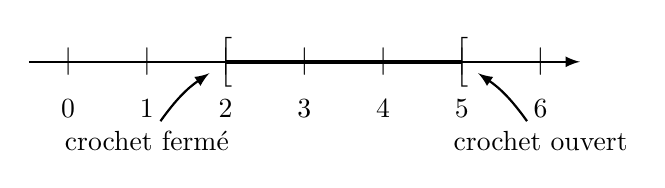
\begin{tikzpicture}[>=latex,baseline={([yshift=-.5ex]current bounding box.center)}]
    \draw[thick,->] (-0.5,0) --(6.5,0);
    \node[] (2) at (2,0) {$\textbf{\Big[}$};
    \node[] (5) at (5,0) {$\Big[$};
    \node[] (cf) at (1,-1) {crochet fermé};
    \node[] (co) at (6,-1) {crochet ouvert};
    \draw[ultra thick,-] (2,0) --(5,0);
    \foreach \xp in {0,1,...,6}{\node[] at (\xp,0) {$\mid$};}
    \foreach \xp in {0,1,...,6}{\node[below=10pt] at (\xp,0) {\xp};}
    \draw[->,>=latex,thick] (cf) to[bend left=10] (2);
    \draw[->,>=latex,thick] (co) to[bend right=10] (5);
\end{tikzpicture}
\vspace{1mm}
\item Par une inégalité: $2 \leq x < 5$
\vspace{1mm}
\item Par un intervalle: $[2;5[$
\end{itemize}

Soient $a$ et $b$ deux réels distincts.

\begin{center}
\begin{tabularx}{\textwidth}{ 
  | >{\centering\arraybackslash}c 
  | >{\centering\arraybackslash}X
  | >{\centering\arraybackslash}X | }
\hline
L'intervalle noté $\ldots$ & $\ldots$ désigne l'ensemble des réels $x$ tels que $\ldots$ & Il est représenté par un segment sur une droite graduée\\ \hline 
\large{$\left[ a;b \right]$} & \large{$a \leq x \leq b$} & 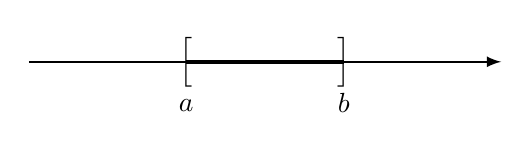
\begin{tikzpicture}[>=latex]
    \draw[thick,->] (0,0) --(6,0);
    \node[] at (2,0) {$\textbf{\Big[}$};
    \node[] at (4,0) {$\Big]$};
    \node[below=10pt] at (2,0) {$a$};
    \node[below=8pt] at (4,0) {$b$};
    \draw[ultra thick,-] (2,0) --(4,0);
\end{tikzpicture} \vspace{-2mm} \\ \hline 
\large{$\left] a;b \right]$} & \large{$a < x \leq b$} & 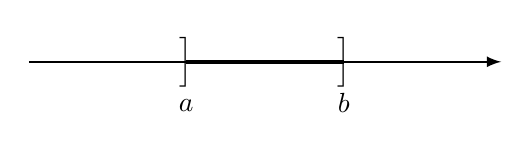
\begin{tikzpicture}[>=latex]
    \draw[thick,->] (0,0) --(6,0);
    \node[] at (2,0) {$\textbf{\Big]}$};
    \node[] at (4,0) {$\Big]$};
    \node[below=10pt] at (2,0) {$a$};
    \node[below=8pt] at (4,0) {$b$};
    \draw[ultra thick,-] (2,0) --(4,0);
\end{tikzpicture} \vspace{-2mm} \\ \hline 
\large{$\left[ a;b \right[$} & \large{$a \leq x < b$} & 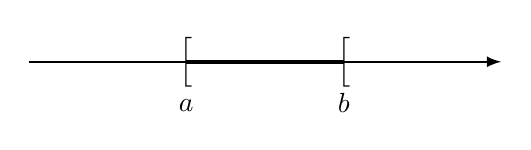
\begin{tikzpicture}[>=latex]
    \draw[thick,->] (0,0) --(6,0);
    \node[] at (2,0) {$\textbf{\Big[}$};
    \node[] at (4,0) {$\Big[$};
    \node[below=10pt] at (2,0) {$a$};
    \node[below=8pt] at (4,0) {$b$};
    \draw[ultra thick,-] (2,0) --(4,0);
\end{tikzpicture} \vspace{-2mm} \\ \hline 
\large{$\left] a;b \right[$} & \large{$a < x < b$} & 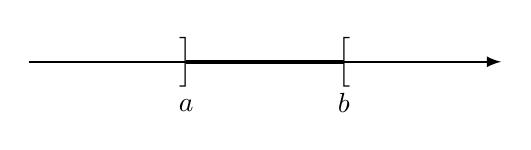
\begin{tikzpicture}[>=latex]
    \draw[thick,->] (0,0) --(6,0);
    \node[] at (2,0) {$\textbf{\Big]}$};
    \node[] at (4,0) {$\Big[$};
    \node[below=10pt] at (2,0) {$a$};
    \node[below=8pt] at (4,0) {$b$};
    \draw[ultra thick,-] (2,0) --(4,0);
\end{tikzpicture} \vspace{-2mm} \\ \hline 
\large{$\left] - \infty;b \right]$} & \large{$x \leq b$} & 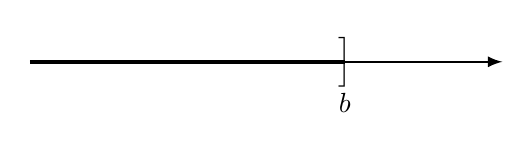
\begin{tikzpicture}[>=latex]
    \draw[thick,->] (0,0) --(6,0);
    \node[] at (4,0) {$\Big]$};
    \node[below=8pt] at (4,0) {$b$};
    \draw[ultra thick,-] (0,0) --(4,0);
\end{tikzpicture} \vspace{-2mm} \\ \hline 
\large{$\left] - \infty;b \right[$} & \large{$x < b$} & 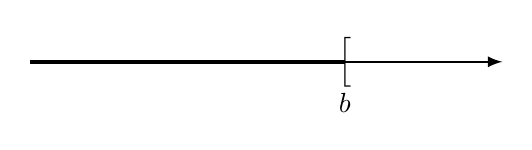
\begin{tikzpicture}[>=latex]
    \draw[thick,->] (0,0) --(6,0);
    \node[] at (4,0) {$\Big[$};
    \node[below=8pt] at (4,0) {$b$};
    \draw[ultra thick,-] (0,0) --(4,0);
\end{tikzpicture} \vspace{-2mm} \\ \hline 
\large{$\left[ a;+ \infty \right[$} & \large{$a \leq x $} & 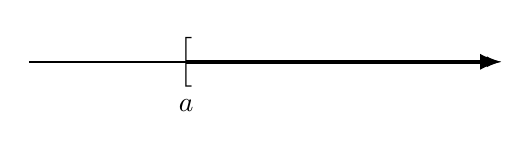
\begin{tikzpicture}[>=latex]
    \draw[thick,->] (0,0) --(6,0);
    \node[] at (2,0) {$\textbf{\Big[}$};
    \node[below=10pt] at (2,0) {$a$};
    \draw[ultra thick,->] (2,0) --(6,0);
\end{tikzpicture} \vspace{-2mm} \\ \hline 
\large{$\left] a; + \infty \right[$} & \large{$a < x$} & 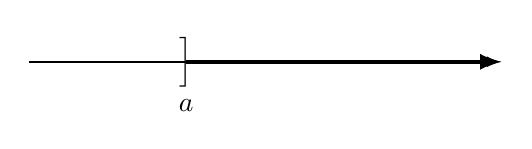
\begin{tikzpicture}[>=latex]
    \draw[thick,->] (0,0) --(6,0);
    \node[] at (2,0) {$\textbf{\Big]}$};
    \node[below=10pt] at (2,0) {$a$};
    \draw[ultra thick,->] (2,0) --(6,0);
\end{tikzpicture} \vspace{-2mm} \\ \hline
\end{tabularx}
\end{center}
\end{defin}

\begin{rmqs} \begin{itemize}
\item $a$ et $b$ sont appelés les bornes de l'intervalle.
\item Attention à ne pas confondre $\left[a;b\right] et \left\{a;b\right\}$: Le premier ensemble contient tous les réels compris entre $a$ et $b$ inclus, alors que le second ne contient que $a$ et $b$.
\item $- \infty$ et $+ \infty$ ne sont pas des nombres réels, on écrit donc pas $\left[- \infty ; a \right]$.
\item $\R = \left] - \infty ; + \infty \right[$
\item Les quatre premiers intervalles sont dits bornés. Parmi ceux-ci, on dit que $\left[a;b\right]$ est fermé, $\left]a;b\right[$ est ouvert. Les deux autres sont dits semi-ouverts.
\end{itemize}
\end{rmqs}

\subsection*{Unions et intersections}

\begin{defin}
Soient $I$ et $J$ deux intervalles de $\R$.
\begin{itemize}
\item L'ensemble des réels qui appartiennent à la fois à $I$ et à $J$ est appelé intersection de $I$ et $J$. Cet ensemble est noté $I \cap J$.

\item L'ensemble des réels qui appartiennent à à $I$ ou à $J$ est appelé réunion de $I$ et $J$. Cet ensemble est noté $I \cup J$.

\end{itemize}
\end{defin}

\begin{ex}
Pour $I=[-2;3[$ et $J=[-4;1]$, on a $I \cap J = [-2;1]$ et $I \cup J = ]-4;3[$.

\begin{center}
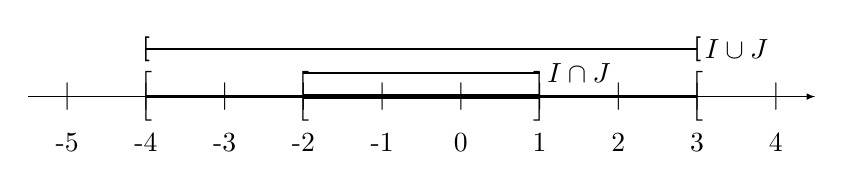
\begin{tikzpicture}[>=latex]
    \draw[ultra thin,->] (-5.5,0) --(4.5,0);
    \draw[thick,-] (1,0) --(3,0);
    \draw[thick,-] (-4,0) --(-2,0);
    \draw[ultra thick,-] (-2,0) --(1,0);
    \foreach \xp in {-5,-4,...,4}{\node[] at (\xp,0) {$\mid$};}
    \foreach \xp in {-5,-4,...,4}{\node[below=10pt] at (\xp,0) {\xp};}
    \node[] at (-2,0) {$\textbf{\Big[}$};
    \node[] at (3,0) {$\textbf{\Big[}$};
    \node[] at (-4,0) {$\textbf{\Big[}$};
    \node[] at (1,0) {$\textbf{\Big]}$};
    \draw[thick,-] (-2,0.3) --(1,0.3);
    \draw[thick,-] (-4,0.6) --(3,0.6);
    \node[] at (1.5,0.3) {$I \cap J$};
    \node[] at (3.5,0.6) {$I \cup J$};
	\node[] at (-4,0.6) {$\textbf{\small[}$};
	\node[] at (3,0.6) {$\textbf{\small[}$};
   
\end{tikzpicture}
\end{center}

\end{ex}
\rem{Exo}

\section{Valeur absolue}

\begin{defin}
La valeur absolue d'un réel $x$ est $-x$ lorsque $x<0$ ou $x$ lorsque $x \geq 0$. On note: $$\vert x \vert = \left\{ \begin{aligned} -x \text{ si } x < 0 \\ x \text{ si } x \geq 0 \end{aligned} \right.$$
\end{defin}

\begin{ex}
$\abs 8 = 8$ mais $\abs {-8} = 8$ aussi. En fait, l'effet de la valeur absolue est de rendre un nombre positif ( on supprime le signe $-$ ).
\end{ex}

\begin{defin}
Soient $A$ et $B$ deux points placés sur la droite des réels, d'abscisses respectives $a$ et $b$. La distance entre $a$ et $b$ correspond à la longueur de $AB$. Elle se calcule à l'aide de la valeur absolue:
$$AB = \abs{b-a} = \abs{a-b}$$
\end{defin}

\begin{ex}
\begin{itemize}
\item La distance entre $5$ et $-2$ est $\abs{5 - (-2)} = \abs{5+2} = \abs 7 = 7$.
\item Soit $x \in \R$. La distance entre $x$ et $0$ est $\abs{x-0} = \abs x$.
\end{itemize}
\end{ex}

\subsection*{Intervalles $[a-r;a+r]$}

\begin{propr}
Soient $a$ et $r$ deux réels, avec $r > 0$. Alors l'intervalle $[a-r;a+r]$ contient tous les réels $x$ qui vérifient $a-r \leq x \leq a+r$, autrement dit ceux à une distance inférieure à $r$ de $a$, soit $\abs {x-a} \leq r$.
\end{propr}

\begin{ex}
$[3;5]=[4-1;4+1]=\left\{ x \in \R, \ \abs{x-4} \leq 1 \right\}$
\end{ex}

\rem{Démonstration de $\frac 1 3$ non décimal}

\begin{comment}

\begin{center}
\begin{tikzpicture}
\begin{axis}[
axis x line=bottom,
axis y line = left,
axis lines=middle,
width=\linewidth,
xmin=-5, xmax=5,
%ymin=-5, ymax=20,
%enlargelimits=true,
%xlabel=$x$,
ylabel={$f(x) = x^2$},
minor x tick num=1,
minor y tick num=4,
%ytick distance=1,
grid=major,
grid style=dashed,
axis equal,
]
\addplot[smooth]{x^2};
\addplot[smooth,domain=0:14]{ln(x)};

\end{axis}
\end{tikzpicture}
\end{center}

\begin{center}
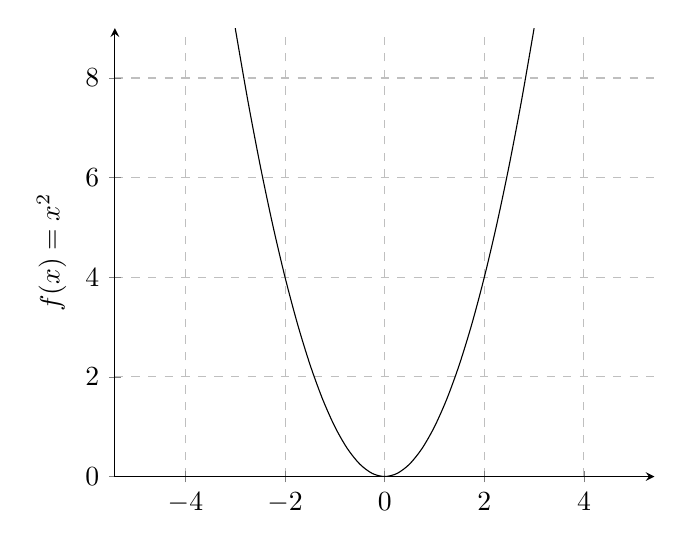
\begin{tikzpicture}
\begin{axis}[
axis x line=bottom,
axis y line = left,
%enlargelimits=true,
%xlabel=$x$,
ylabel={$f(x) = x^2$},
grid=major,
grid style=dashed,
axis equal,
]
%
use TeX as calculator:
\addplot[domain=-3:3,smooth] {x^2};
\end{axis}
\end{tikzpicture}
\end{center}

\end{comment}


\end{document}
